\documentclass[CJK]{ctexart}
\usepackage{CJK}
\usepackage{amsmath}
\usepackage{listings}
\CTEXsetup[format={\Large\bfseries}]{section}
\usepackage{graphicx}
\usepackage{lastpage}
\usepackage{float}
\usepackage[superscript]{cite}
\usepackage{geometry}
\usepackage{bm}
\usepackage{enumerate}
\usepackage{subfigure}
\usepackage{algorithm}  
\usepackage{algorithmicx}  
\usepackage{algpseudocode} 
\usepackage{setspace}
\pagestyle{plain}
\geometry{left=1.8cm,right=1.8cm,top=1.5cm,bottom=2cm}

\floatname{algorithm}{算法}  
\renewcommand{\algorithmicrequire}{\textbf{输入:}}  
\renewcommand{\algorithmicensure}{\textbf{输出:}}  

\begin{document}
\title{\textbf{问题求解与实践 \quad 课程作业}}
\author{518030910092 谢哲}
\date{}
\maketitle

\begin{abstract}
    在本作业中,使用C++对kaggle中的共享自行车使用情况数据集进行了分析。首先,使用一个特定的类对数据进行读取和存储,并剔除了不符合条件的脏数据。使用FLTK对数据使用折线图、饼状图、比例图、柱状图等进行可视化。最后,使用\textbf{自己编写的神经网络框架}和多元线性回归方法,分别根据环境对自行车使用情况进行了预测,神经网络的预测方法效果良好。\textbf{报告的最后给出了demo的使用方法。}
\end{abstract}
\section{数据读入}
\subsection{任务描述}
    该数据集存储了某城市2011和2012年的每小时、每天的共享自行车的使用量,和当时的日期、时间、季节、节假日、工作日、温度、湿度、天气、注册用户数、非注册用户数等数据。
\subsection{解决方案}
为了将数据读入进行分析与预测,首先进行如下三个步骤对数据进行读入与预处理。
    \begin{enumerate}[(1)]
        \item \textbf{数据读入}\quad 在数据读入部分中,使用了一个\textbf{Data\_Reader}类处理数据的读入。并将原始的.csv数据使用fstream读入并以逗号分割后,将不同类别的数据以字符串方式存储,以字符串向量的方式存入一个raw\_data向量容器中。
        \item \textbf{脏数据处理}\quad 读入原始数据后先进行脏数据处理,脏数据处理的具体方法详见第2节。
        \item \textbf{数据存储}\quad 在处理脏数据之后,进入数据读取步骤。在Data\_Reader类中,定义了一个类Bikie\_Data来存储不同格式的数据,包括日期、天气、温度、用户量等。并将所有剔除脏数据后的raw\_data数据输入格式转换函数,将字符串类别转化为相应的特定类别数据,存入Bike\_Data类变量,装入Bike\_Data类别的processed\_data向量容器中。以线性方式完成数据集的存储。
    \end{enumerate} 
\subsection{结果}
数据集中的两个数据文件data.csv和hour.csv均能被正常读取并存入向量容器内。容器内的数据可以被快速、方便地访问和查找,为之后的可视化和数据预测提供了有力的支持。
\section{脏数据处理}
\subsection{任务描述}
该共享自行车数据集提供了包括日期、相对温度、相对湿度、季节、天气和使用量等多方面的信息。而在此之中可能包括各种各样的脏数据,包括格式不正确、数据范围不合理、数据自相矛盾和数据本身没有实际价值等多方面的情况,需要将其进行脏数据处理之后,再进行可视化和数据预测的操作,避免脏数据带来的影响。
\subsection{解决方案}
对于数据集中的每一条记录,由于数据类型多种多样,而且表达的意义不同,所以不可能使用统一的方法来确定所有数据的脏数据标准。因此必须对于每一类别的数据分别定义脏数据标准。经过对数据的整体分析,确定的脏数据标准如下。\par
对于序号类别,由于其在可视化和预测中不起到任何作用,所以一律删除;对于日期类别,需确定其格式是否正确;对于季节、年份、月份、节假日、时间、工作日和天气状况类别,需保证其数据范围在数据集给定的范围之内;对于相对温度和体感相对温度,由于体感温度更具实际价值,仅保留体感相对温度;对于相对湿度,其正常范围均处于$0.1\sim1.0$之间,剔除之外的部分;对于用户总数、非注册用户数和注册用户数,需保证总数等于非注册和注册数量之和的客观规律。对于其余类别数据,需保证输入格式正确。对于任何非法数据(即不符合前述要求的数据),由于无法恢复,\textbf{应当直接剔除该条记录}。
\subsection{结果}
经过程序对源数据的格式筛选和格式化数据的数值筛选后,共剔除了26条脏数据。剔除了脏数据之后,数据被直接保存在processed\_data向量容器中,为之后的可视化和数据预测的有效性和准确性提供了必不可少的前提条件。
\section{数据可视化}
\subsection{任务描述}
    数据集一共包含了包含时间、用户数量、天气、温度等多个维度的近20000条数据,并且数据间可能存在一定的关联性。为了将这些数据以更直观的方式展现出来,可以使用FLTK库,采用数据可视化的方法来清晰地展现这些数据的某些特点。
\subsection{解决方案}
    对于该数据集,存在多种数据可视化方法,包括条形图、折线图、饼状图、比例图等,而且每种类别的图形均被使用了多次。考虑使用面向对象的方式,将每种类别的图都写为一个类。为了使用方便,这些类都继承了课程中使用的Graph.h中的Shape类,可以使用统一的方式绑定到Simple\_Window.h中的Simple\_Window显示。再统一通过Show\_Data类进行封装,方便用户调用。\par
    
    在每个类中,重载了draw\_lines函数,并且根据数据可视化方法的实际情况,增加了其它的一些函数进行重载。例如,在折线图中增加了设定坐标轴标签和范围的函数,在饼状图中增加了设定系列标签的函数等。可视化部分的继承和调用结构如图\ref{fig:struct_vision}所示。相较于FLTK自带的Fl\_Chart类,自定义的可视化图标类可以同时显示多个系列的折线图,并且有更为准确的数据标签,功能更为丰富,生成的图表更为美观。\par

    \begin{figure}[htbp]
        \centering
        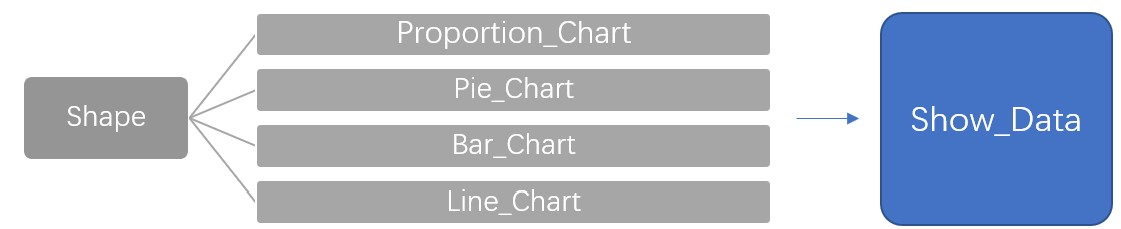
\includegraphics[width=5in]{img/struct_1.jpg}
        \caption{可视化部分结构}
        \label{fig:struct_vision}
    \end{figure}

    对于每日的用户量的变化情况,使用折线图来展示,并使用不同的颜色来区分不同的系列(注册、未注册、总数量),如图\ref{fig:year}所示。对于注册于未注册用户的比例情况,使用饼状图来反应,并使用比例图来反应其随着时间的比例变化情况。对于每天各时段的用户,使用折线图来反应其随时间的变化情况。对于不同气候条件下的用户数量,使用折线图和条形图进行可视化。
    
\subsection{结果}
    由于篇幅有限,下图中仅展示部分可视化图片,全部可视化结果可以按照文末的说明运行demo查看。通过这些数据,不难分析出随着时间、温度变化,用户数量和比例的变化。
    
    \begin{figure}[htbp]
        \centering
        \subfigure[每日各类别用户量折线图]{
        \begin{minipage}[t]{0.33\linewidth}
        \centering
        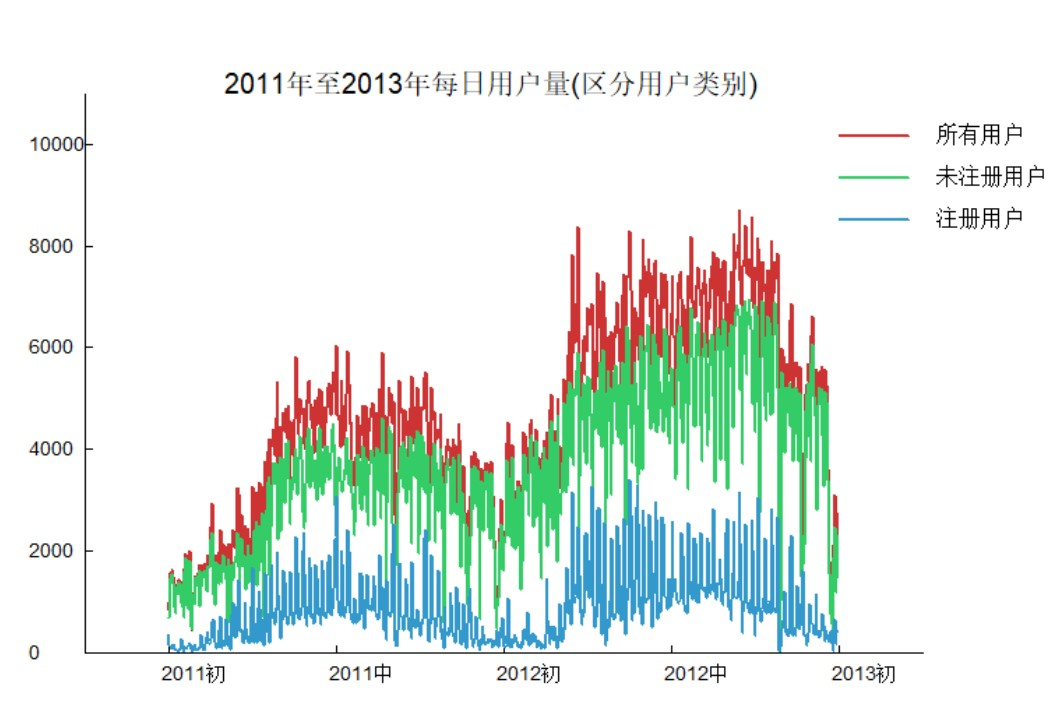
\includegraphics[width=2.3in]{img/year_2.jpg}
        %\caption{fig1}
        \end{minipage}%
        }%
        \subfigure[不同温度用户量折线图]{
        \begin{minipage}[t]{0.33\linewidth}
        \centering
        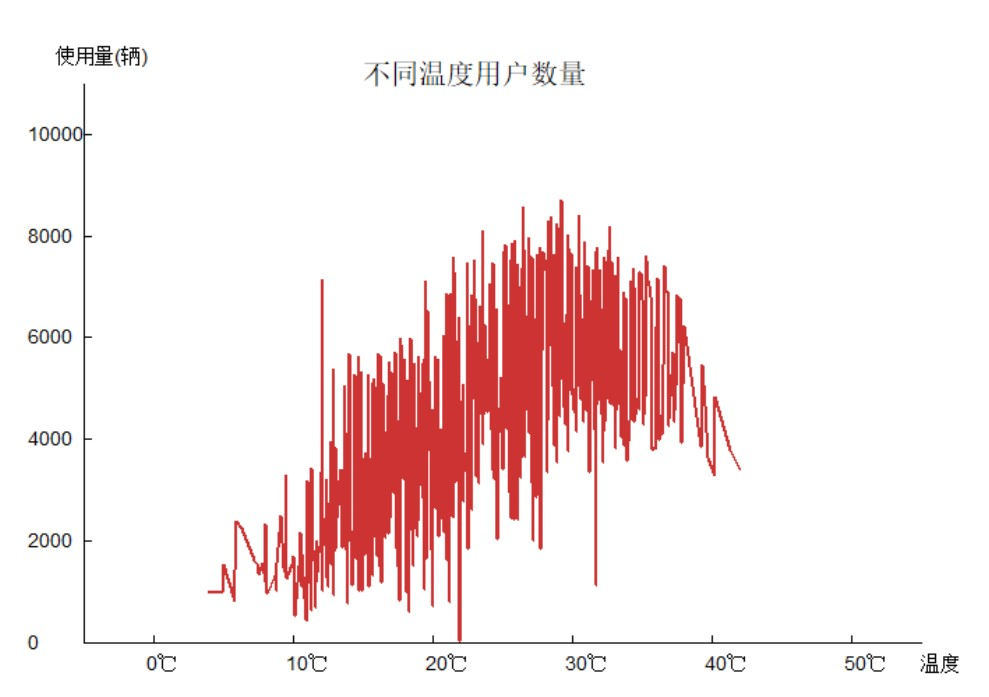
\includegraphics[width=2.3in]{img/temp_1.jpg}
        %\caption{fig2}
        \end{minipage}%
        }%
        \subfigure[每小时平均用户数量变化折线图]{
        \begin{minipage}[t]{0.33\linewidth}
        \centering
        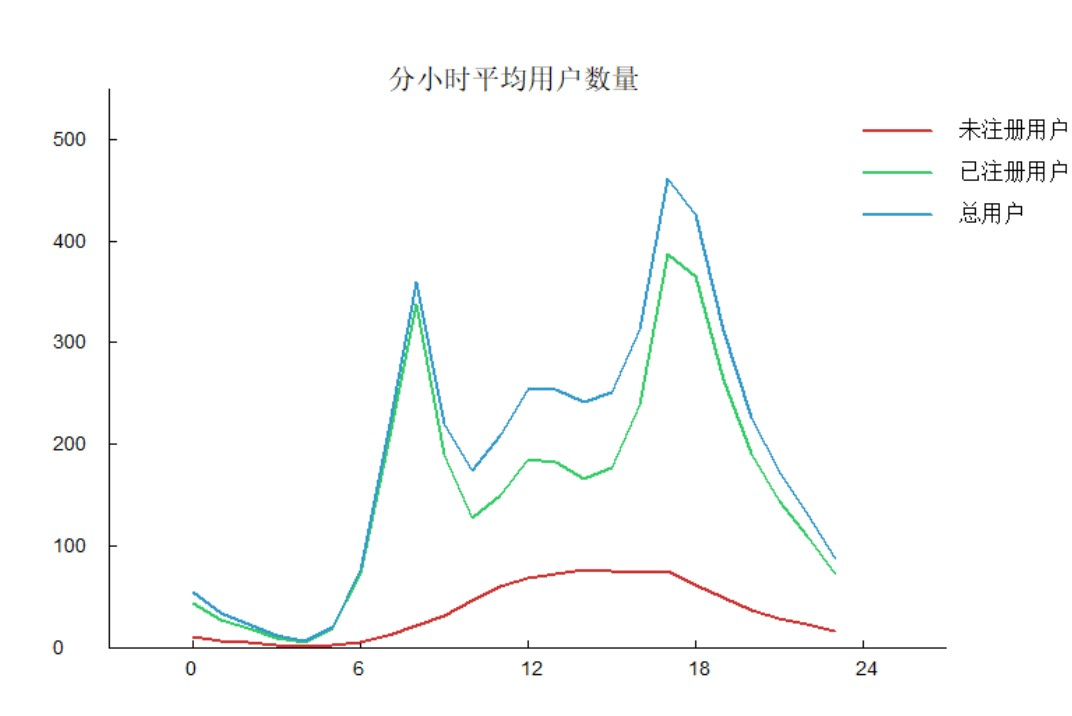
\includegraphics[width=2.5in]{img/day_1.jpg}
        %\caption{fig2}
        \end{minipage}%
        }%
        \centering
        \caption{折线图}
        \label{fig:year}
    \end{figure}
    
    \begin{figure}[htbp]
        \centering
        \subfigure[用户比例饼状图]{
        \begin{minipage}[t]{0.25\linewidth}
        \centering
        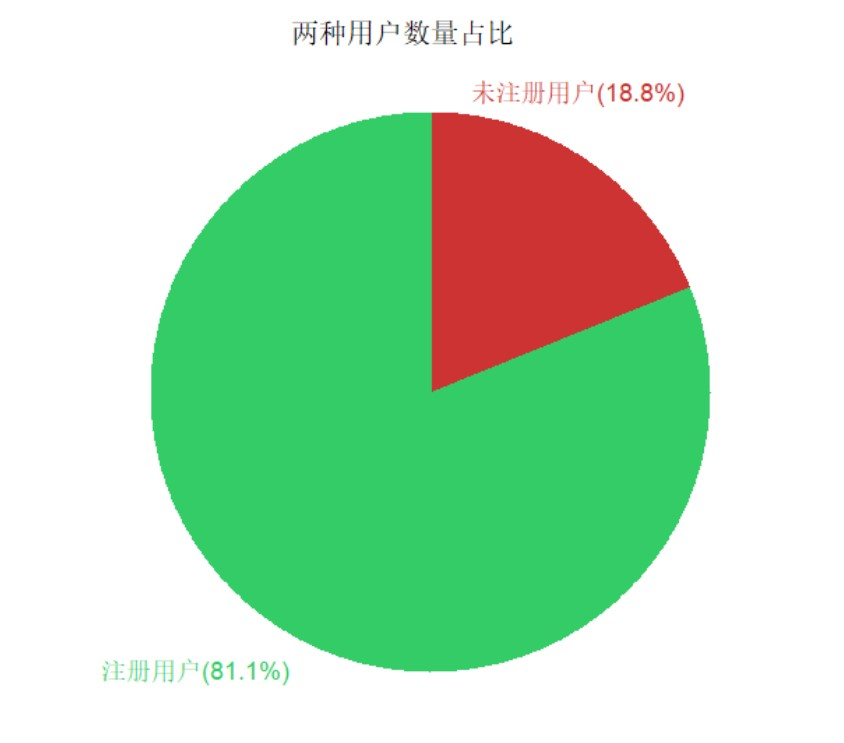
\includegraphics[width=1.5in]{img/pie_1.jpg}
        %\caption{fig1}
        \end{minipage}%
        }%
        \subfigure[不同天气的用户数量条形图]{
        \begin{minipage}[t]{0.25\linewidth}
        \centering
        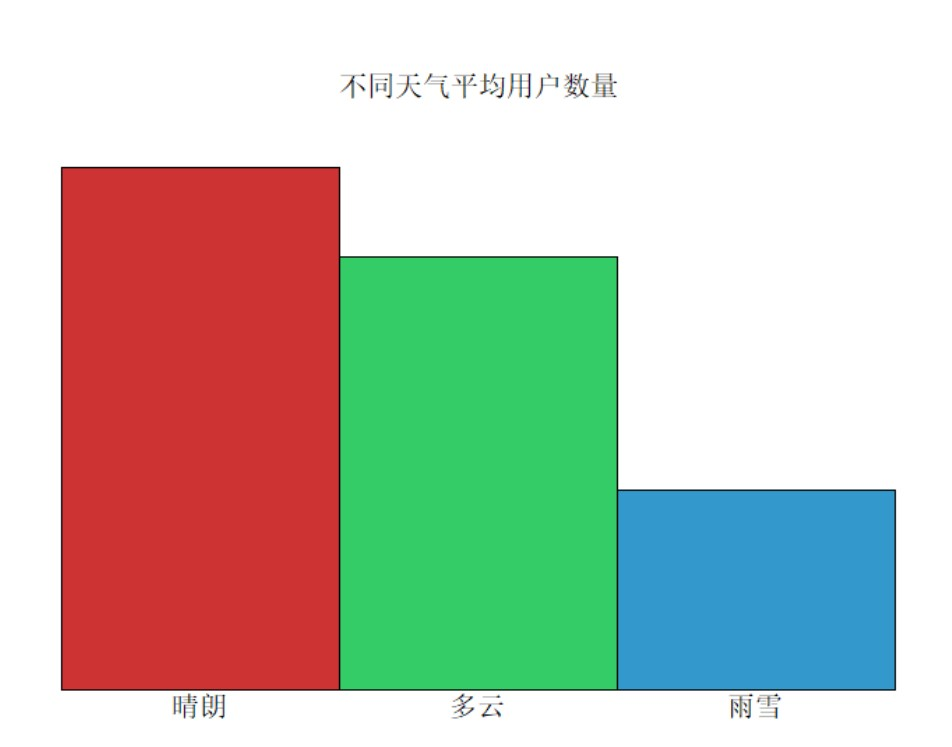
\includegraphics[width=1.7in]{img/bar_1.jpg}
        %\caption{fig2}
        \end{minipage}%
        }%
        \subfigure[每周各日用户比例变化比例图]{
        \begin{minipage}[t]{0.5\linewidth}
        \centering
        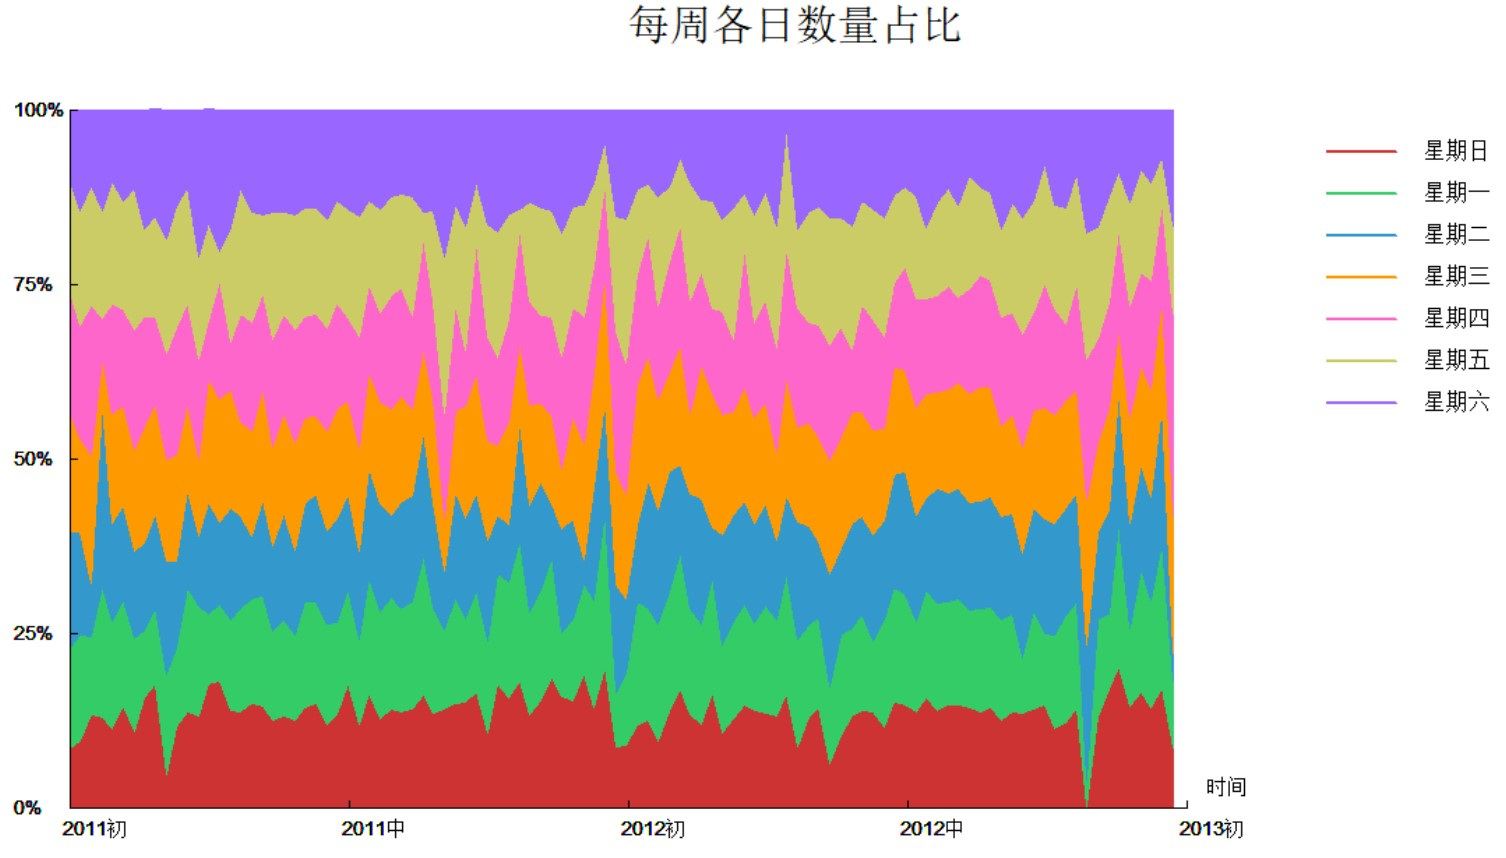
\includegraphics[width=2.8in]{img/proportion_2.jpg}
        %\caption{fig2}
        \end{minipage}%
        }%
        \centering
        \caption{饼状图、条形图和比例图}
    \end{figure}

\section{数据预测}
\subsection{任务描述}
本数据集的预测目标是共享自行车的总使用人数。预测的依赖因素包括年份、月份、天气、温度和湿度等信息。由于年份等与时间相关的因素是客观已知的,且天气、温度和湿度等信息是可以通过天气预报技术预测的,所以根据这些信息预测出当天的总单车使用量具有一定的可行性和实用价值。根据当初设定的目标,先根据随机划分的数据集与测试集,在预测模型生成之后,将对所有两年的每日使用数据与每小时使用数据进行预测。之后将前7个季度划分为数据集,后1个季度作为测试集,预测最后一个季度的每日单车使用情况。
\subsection{解决方案}
由于本任务存在多个因素,所以使用之前所学的一元线性回归等一元拟合方法是不可行的。于是考虑采用多元线性回归和神经网络的方法进行拟合。
\begin{enumerate}[(1)]
    \item \textbf{多元线性回归}\quad 多元线性回归与一元线性回归类似。对于其中的一个样本 $(x_1,x_2,\cdots,x_n)$,其对应的多元线性回归值为$\hat{y}=b_0+b_1x_1+b_2x_2+\cdots+b_nx_n$,其原理为优化参数$ \hat{b_i} $,最小化这些参数表述的回归超平面上的预测值与真实值的残差平方和$Q(b_0,b_1,\cdots,b_n)$。通过数学方法,可以得到如下的线性方程组,可以求得参数的理论值。
    \begin{gather*}
    b_0=\overline{y}-b_1\overline{x_1}-b_2\overline{x_2}-\cdots-b_n\overline{x_n}\\
    s_{11}b_1+s_{12}b_2+\cdots+s_{1n}b_n=s_{1y}\\
    \cdots\\
    s_{n1}b_1+s_{n2}b_2+\cdots+s_{nn}b_n=s_{ny}
    \end{gather*}
    其中$s_{jk}=\sum\limits_{i=1}^n(x_{ji}-\bar{x_j})(x_{ki}-\bar{x_k}),s_{jy}=\sum\limits_{i=1}^n(x_{ji}-\bar{x_j})(y_i-\bar{y})$。将实际值通过公式计算,代入线性方程组,使用高斯消元法求解,即可得到结果。
    \item \textbf{神经网络}\quad 由于在本数据集中,各种因素与最终结果的关系不一定是线性关系,所以需要进行多元函数的高次拟合,神经网络便是这样一种能够拟合多元高次函数的简洁、高效的方法。直接调用一些线程的机器学习库进行训练不是本课程的初衷,于是考虑\textbf{从零实现一个简单易用的C++神经网络框架},对数据进行预测。\par
    \begin{figure}[htbp]
        \centering
        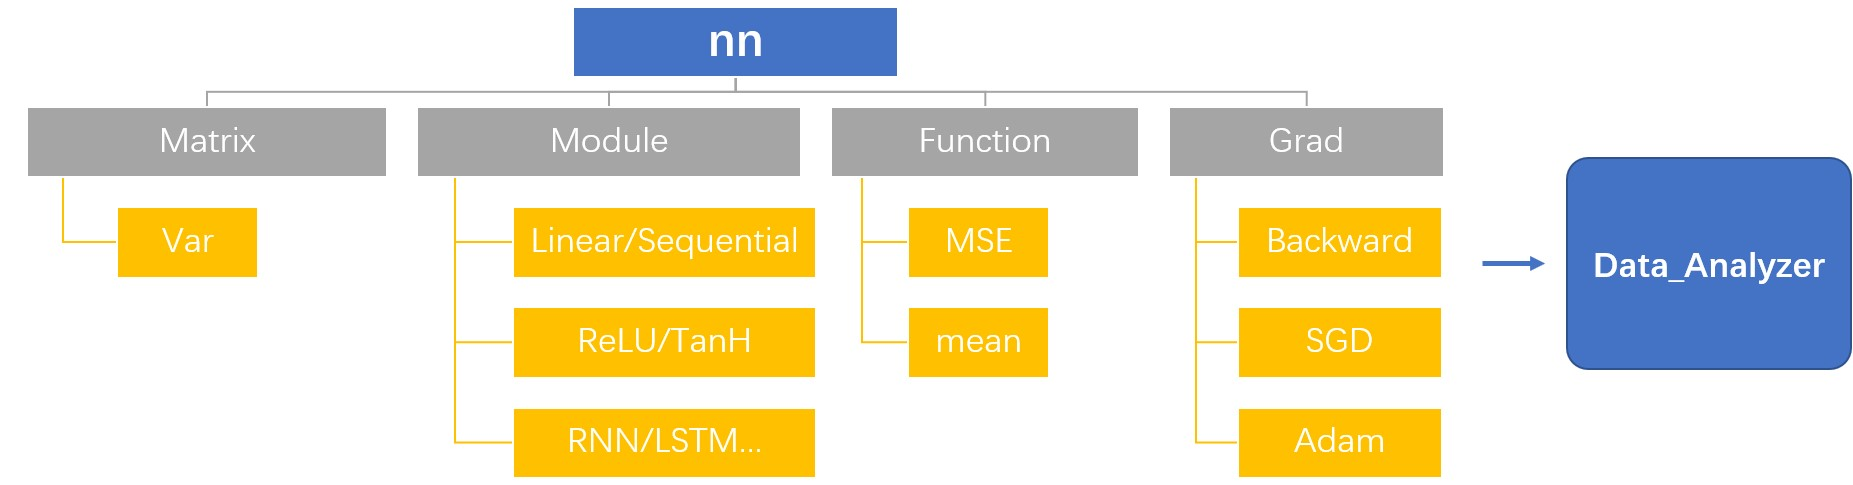
\includegraphics[width=6in]{img/struct_2.jpg}
        \caption{神经网络框架结构}
        \label{fig:struct_nn}
    \end{figure}
    \qquad 本人实现的神经网络框架为静态神经网络,它的结构如图\ref{fig:struct_nn}所示。所有的类和函数都被包括在了一个名为nn的namespace中,这些类的结构全部声明在nn.h中方便查阅。由于神经网络运算本质是矩阵运算,所以定义了一个Matrix类完成矩阵的基本运算,这部分的内容定义在nn\_matrix.cpp中。Var类为神经网络计算图的基本单元,内部结合了Matrix类,记录了结点数据、梯度数据、优化器参数和计算图中的子节点的指针,并提供了backward函数和optim函数以进行反向传播和参数优化,这部分的内容定义在nn\_var.cpp中。\par
    \qquad 为了方便用户实现计算图的快速搭建,神经网络框架充分使用C++11中的特性。例如,为了防止作用域内的结点在作用域外被析构,从而导致计算图失效,使用智能指针std::shared\_ptr实现堆内存管理,保证所有计算图结点在运行过程中始终有效;为了使得多项式计算过程中,右值计算结果不失效,定义了移动赋值函数和右值引用类型的重载函数。\par
    \qquad 由于计算图的构建,前向传播和反向传播的过程是简单的,只需使用DFS遍历计算图,递归计算前向传播值和梯度值即可。Module模块内置了Linear、RNN、LSTM等常用网络结构和ReLU、TanH、Sigmoid等激活函数,并提供了Sequential类来将这些结构顺序串联起来,完成神经网络的快速搭建。Module模块内置了一个forward函数,包括了前向传播的计算过程,不同的框架模块只需修改其前向传播过程即可,这个过程是简单的,只需要根据现有的相关资料和论文得到各种神经网络的计算公式即可。反向传播之后,使用SGD或Adam优化器即可优化权重参数,以训练神经网络。反向传播和优化器的部分定义在nn\_grad.cpp中。\par
    \qquad 在训练每日用户数据预测过程中,使用的网络结构为4层全连接神经网络,输入层神经元个数为特征数(8个或9个,视具体训练数据而定);第一隐藏层神经元个数为32,激活函数为ReLU;第二隐藏层神经元个数为64,激活函数为ReLU;输出层神经元个数为1。在训练每小时数据预测过程中,为增强其学习能力,增加为6层神经网络。\par
    \qquad 经过实验发现Adam优化器收敛速度更快,效果更佳,于是在训练过程中使用Adam优化器进行优化。其简化后的伪代码如下:
    \begin{algorithm}
        \caption{Adam优化器}
        \begin{spacing}{1.1}
        \begin{algorithmic}[1]
            \Require $\textbf{学习率}\alpha,\beta_1,\beta_2,\textbf{函数}f(\theta),\textbf{初始参数}\theta_0$
            \State $m_0\leftarrow0,v_0\leftarrow0,t\leftarrow0$
            \While{$\theta_t$更新}
            \State $t\leftarrow t+1$
            \State $g_t\leftarrow \nabla_\theta f_t(\theta_{t-1})$
            \State $m_t\leftarrow \beta_1\cdot m_{t-1}+(1-\beta_1)\cdot g_t$
            \State $v_t\leftarrow \beta_2\cdot v_{t-1}+(1-\beta_2)\cdot g_t^2$
            \State $\hat{m_t}\leftarrow m_t/(1-\beta_1^t)$
            \State $\hat{v_t}\leftarrow v_t/(1-\beta_2^t)$
            \State $\theta_t\leftarrow \theta_{t-1}-\alpha\cdot\hat{m_t}/(\sqrt{\hat{v_t}}+\epsilon)$
            \EndWhile
            \State \Return $\theta_t$
        \end{algorithmic}    
        \end{spacing}
    \end{algorithm}
\end{enumerate}\par
在得到预处理的数据之后,为了进行多元线性回归或神经网络训练,需要项将其先强制转化为double类型的向量。其中,每小时的数据和每日的数据相比,要多出一个“时间”变量,所以预测时的输入需要多出一个维度。在确定输入、输出向量之后,根据任务描述中的要求划分训练集和测试集。随机划分时,按照9:1的比例划分训练集与测试集。之后将训练集放入定义好的神经网络内训练,训练集经过随机排序后,按照每批100个放入网络前向与反向传播。损失函数采用误差率,优化器采用Adam,学习率设定为0.005。最后评判在测试集上的误差率,(由于实际情况,将原任务描述中的准确率评判变为误差率评判),误差率的定义如下:
$$\mbox{误差率}=\min(\frac{|\mbox{当日预测用车次数}-\mbox{当日实际用车次数}|}{\mbox{当日实际用车次数}},1)\times 100\%$$
\subsection{结果}
\subsubsection{随机划分预测每日数据}
使用最小二乘法预测每日总用车辆在测试集上的误差率为18.87\%;使用神经网络预测每日总用车辆在测试集上的误差率为16.39\%,预测结果优于最小二乘法的预测结果。为了体现其训练效果,图\ref{fig:loss_1}展示了随机划分训练集和测试集情况下,随着训练轮数的增加的误差率的变化情况和在预测集上两种不同方法的预测表现。可以发现,随着训练轮数的增加,神经网络的误差率逐渐减小,最终低于最小二乘法的误差率。而在预测集上的表现可以发现二者都能较好地拟合预测集上的数据,且神经网络在大多数情况下都要略胜一筹。

\begin{figure}[htbp]
    \centering
    \subfigure[训练损失随轮数变化情况]{
    \begin{minipage}[t]{0.5\linewidth}
    \centering
    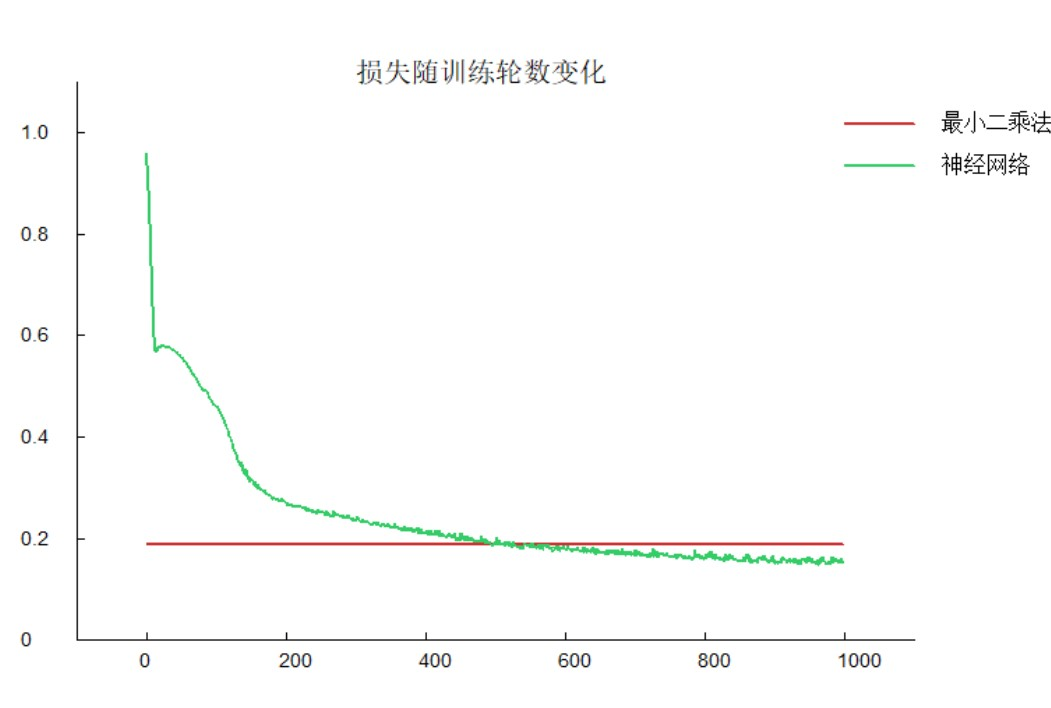
\includegraphics[width=3.5in]{img/loss_1.jpg}
    %\caption{fig1}
    \end{minipage}%
    }%
    \subfigure[预测情况与真实情况比较]{
    \begin{minipage}[t]{0.5\linewidth}
    \centering
    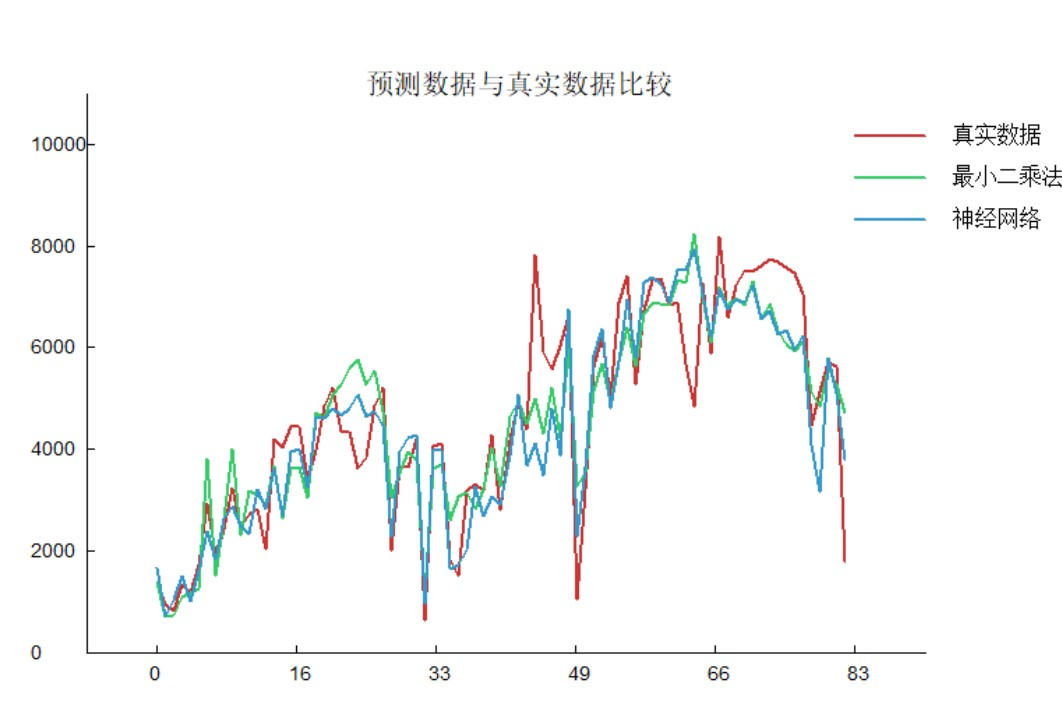
\includegraphics[width=3.5in]{img/loss_2.jpg}
    %\caption{fig2}
    \end{minipage}%
    }%
    \centering
    \caption{随机训练集下的预测情况}
    \label{fig:loss_1}
\end{figure}
\subsubsection{预测最后一个季度的使用情况}
预测最后一个季度的使用情况时,使用最小二乘法的误差率为26.16\%,使用神经网络的误差率为29.61\%,略高于最小二乘法的误差率。然而,根据训练时输出的损失率,可以发现其在测试集上的损失远小于该数字,这也说明神经网络预测时可能存在过拟合的情况。
\subsubsection{预测每天内各小时的使用情况}
使用最小二乘法的误差率为59.98\%,使用神经网络的误差率为28.75\%,远优于最小二乘法。从图\ref{fig:loss_2}(b)中的预测结果与真实结果比较情况,可以发现最小二乘法的拟合曲线更趋向于线性,而神经网络的拟合曲线则是明显是非线性的,贴近于真实曲线,其学习能力较最小二乘法更强。
\begin{figure}[htbp]
    \centering
    \subfigure[预测最后一个季度用户变化情况]{
    \begin{minipage}[t]{0.5\linewidth}
    \centering
    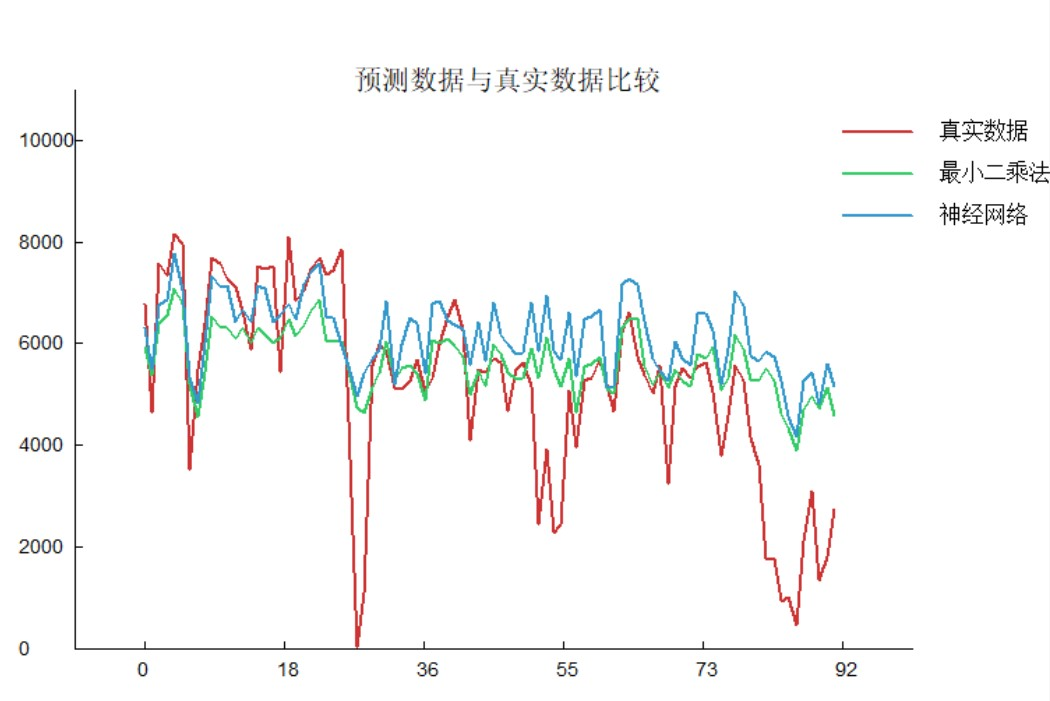
\includegraphics[width=3.5in]{img/loss_3.jpg}
    %\caption{fig1}
    \end{minipage}%
    }%
    \subfigure[预测某天每小时用户变化情况]{
    \begin{minipage}[t]{0.5\linewidth}
    \centering
    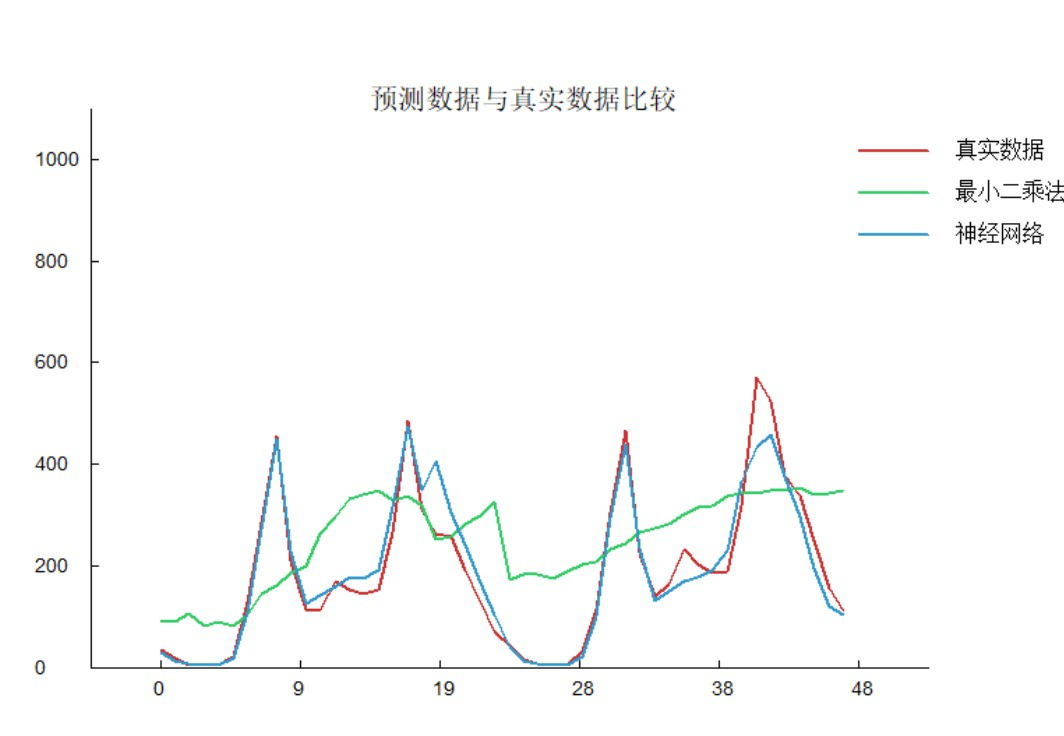
\includegraphics[width=3.5in]{img/loss_4.jpg}
    %\caption{fig2}
    \end{minipage}%
    }%
    \centering
    \caption{特定训练集下的预测情况}
    \label{fig:loss_2}
\end{figure}
\section{Demo使用说明}
\subsection{本文作者的编译和运行环境}
\begin{itemize}
    \item 编译环境:Visual Studio 2019,C++14,fltk-1.3.5,x86,Release。
    \item 运行环境:Windows 10,Intel Core i7-8th,8GB RAM。
\end{itemize}
\subsection{运行步骤}
\begin{enumerate}
    \item 数据读入和脏数据处理:编译并运行程序后,即自动读入全部数据,并且立即自动完成脏数据的处理。
    \item 可视化:按照提示,输入1,按下回车,根据提示选择需要查看的可视化图像。查看完成后,点击窗口右上角的Button,即可返回选择界面。
    \item 数据预测:按照提示,输入2,按下回车,根据提示选择需要预测的数据内容。等待一段时间后会自动弹出预测的误差率结果。
\end{enumerate}

\section{总结}
通过实现数据集的读入、脏数据处理、可视化和数据预测,我学习了许多数据处理和可视化方面的实用的技巧。如今是大数据时代,对数据分析的能力非常重要。通过这次大作业,我加深了对数据分析的理解和认识。\par
此外,通过实现FLTK可视化和自己手动实现神经网络框架的过程,我认识到了一个好的程序框架对于程序的可维护性和可扩展性的重要意义。相比于重构的时间,在写代码之前认真思考程序的框架,能够起到事半功倍的神奇效果。\par
通过这次的作业,我还认识到神经网络并非万能的。当然在多数情况下,它比一些线性拟合方法得到的结果要更有,但是它也存在过拟合、训练速度慢等问题。例如在第2个任务中,神经网络的预测结果甚至不如最小二乘法的预测结果;但是在最后一个任务中,由于预测的曲线明显是非线性的,所以神经网络的预测结果远远优于最小二乘法的预测结果。这说明我们需要依据实际情况,选择合适的数据预测的方法。

\section{致谢}
感谢在问题求解与实践课上陈雨亭,沈艳艳老师的认真教学和助教课后的耐心辅导。\par
感谢PyTorch开源动态神经网络框架,为本人实现自己的C++神经网络前端提供了思路。

\section{参考文献与相关代码}
[1]PyTorch神经网络框架文档. https://pytorch.org/docs/stable/index.html.\par
[2]本文中作者本人实现的神经网络框架myNN. https://github.com/ligongzzz/myNN. 
\end{document}
